% Créé par Martin Bodin (2012).
% Document sous licence CC BY-NC-SA

% Créé par Martin Bodin (2011).
% Document sous licence CC BY-NC-SA

\documentclass{article}
%\documentclass{scrartcl}

\usepackage{ifxetex}
\ifxetex
\usepackage{xunicode,fontspec,xltxtra}
\else
\usepackage[utf8x]{inputenc}
\usepackage[T1]{fontenc}
\usepackage{amsmath, amsthm}
\usepackage{amsfonts, amssymb}
\fi

\usepackage[francais]{babel}
\usepackage{lmodern}
\usepackage{stmaryrd}
\usepackage{graphicx}
\usepackage[nottoc, notlof, notlot]{tocbibind}
\usepackage[dvipsnames]{pstricks}
\usepackage{pst-circ, pst-plot, pstricks-add}
\usepackage{array}
\usepackage{url}
\usepackage{verse}
\usepackage[colorlinks,linkcolor=black]{hyperref}
\usepackage{ifthen}
\usepackage{longtable, rotating}
%\usepackage{fancyhdr}
\usepackage{fancybox, framed}
\usepackage{textcomp}
\usepackage{marvosym}
%\usepackage{bbding}
%\usepackage{a4wide}
\usepackage{geometry}
%\usepackage{soul}
\usepackage{lettrine}
%\usepackage{yfonts}
\usepackage{oldgerm}
\usepackage{enumerate}
\usepackage{tikz}
\usepackage{dictsym}
\usepackage{pifont}

\ifxetex
\newfontfamily\timesfont[Ligatures=TeX]{Times New Roman}
\setmainfont[Mapping=tex-text, Ligatures={Contextual, Common, Historical, Rare, Discretionary}, Numbers={OldStyle}]{Linux Libertine O}
\fi

%\newcommand{\enluminure}[2]{\lettrine[lines=3]{\small \initfamily #1}{#2}}

\usetikzlibrary{trees}
\usetikzlibrary{arrows,shapes,automata,petri}
\usetikzlibrary{fit}
\usetikzlibrary{calc,decorations.pathmorphing,patterns}


\geometry{
	includeheadfoot,
	margin = 2.54cm,
	top = 1.5cm,
	bottom = 1.5cm
}

\newcommand{\ds}{\displaystyle}

\renewcommand{\ge}{\geqslant}
\renewcommand{\le}{\leqslant}
\renewcommand{\preceq}{\preccurlyeq}
\renewcommand{\succeq}{\succcurlyeq}

\newcommand{\Numero}{\No}
\newcommand{\numero}{\no}

\newcommand{\fixme}{\textbf{FIXME}}

\makeatletter

\newcommand{\defineNewPlayer}[2]{
	\@namedef{couleur#1}{#2}
}

\newcommand{\getPlayerColor}[1]{%
	\@nameuse{couleur#1}%
}

\makeatother

% Des commandes pratiques pour générer le document.
\newcommand{\player}[2]{%
	\ifthenelse{\equal{\forplayer}{y}}{%
		\ifthenelse{\equal{\theplayer}{#1}}%
		{#2}{}%
	}{\begin{barv}[\getPlayerColor{#1}]{2pt}{10pt}#2\end{barv}}%
}
\newcommand{\mj}[1]{%
	\ifthenelse{\equal{\forplayer}{n}}{#1}{}%
}
% Ici suit une commande plus complexe, car plus générale.
\makeatletter

\newcommand{\@beginColor}[3][black]{%
	\ifthenelse{\equal{\forplayer}{n}}{%
		\begin{barv}[#1]{#2}{#3}%
	}{}%
}

\newcommand{\@endColor}{%
	\ifthenelse{\equal{\forplayer}{n}}{%
		\end{barv}%
	}{}%
}


\newcommand{\ignore}[1]{}
\newcommand{\@ident}[3]{%
%	\ifthenelse{\equal{\manyColored}{y}}{#1}{%
%		\marginpar{%
%			#1%
%			\vspace{2cm}%
%			#2%
%		}%
%	}%
	#1%
	\ifthenelse{\equal{\forplayer}{n}}{\@beginColor{0pt}{10pt}}{}%
	#3%
	\ifthenelse{\equal{\forplayer}{n}}{\@endColor}{}%
	#2%
%	\ifthenelse{\equal{\manyColored}{y}}{#2}{%
%		\marginpar{%
%			#1%
%			\vspace{5pt}%
%			#2%
%		}%
%	}%
}

\def\@ouverture#1#2{%
\ifthenelse{\equal{\forplayer}{y}}{}{%
\ifthenelse{\equal{\manyColored}{y}}{\@beginColor[#1]{1pt}{0pt}}{%
\hspace{-1cm}\hspace{-#2mm}\parbox[c][1pt][t]{0pt}{
\begin{tikzpicture}
	\node (a) {};
	\node (b) [right of = a, node distance = 16cm] {};
	\node (c) [below of = a, node distance = 2cm] {};
	\draw [very thick, color = #1] (a.center) -- (b);
	\draw [very thick, color = #1] (a.center) -- (c);
\end{tikzpicture}
}\vspace{-3.2mm}\par%
}%
}%
}
\def\@fermeture#1#2{%
\ifthenelse{\equal{\forplayer}{y}}{}{%
\ifthenelse{\equal{\manyColored}{y}}{\@endColor}{%
\hspace{-1cm}\hspace{-#2mm}\parbox[c][1pt][b]{0pt}{
\begin{tikzpicture}
	\node (a) {};
	\node (b) [right of = a, node distance = 16cm] {};
	\node (c) [above of = a, node distance = 1cm] {};
	\draw [very thick, color = #1] (a.center) -- (b);
	\draw [very thick, color = #1, dashed] (a.center) -- (c);
\end{tikzpicture}
}\vspace{-3.2mm}\par%
}%
}%
}

\def\players@parse#1#2[#3][#4]{%
% #1 :  Suite de \@ouverture
% #2 :  Suite de \@fermeture
% #3 :  Commande à appeler dans le cas d’une réponse négative (≃ réponse précédente).
% #4 :  Argument (sous forme de numéro de joueur) lu actuellement.
	\ifthenelse{\equal{\theplayer}{#4}}{%
		\players@yes{\@ouverture{\getPlayerColor{#4}}{#4}#1}{#2\@fermeture{\getPlayerColor{#4}}{#4}}%
	}{%
		#3{\@ouverture{\getPlayerColor{#4}}{#4}#1}{#2\@fermeture{\getPlayerColor{#4}}{#4}}%
	}%
}

\def\players@no#1#2{%
	\@ifnextchar[{\players@parse{#1}{#2}[\players@no]}{\ignore}%
}

\def\players@yes#1#2{%
	\@ifnextchar[{\players@parse{#1}{#2}[\players@yes]}{\@ident{#1}{#2}}%
}

\def\players{%
	\ifthenelse{\equal{\forplayer}{y}}{%
		\players@no{}{}%
	}{%
		\players@yes{}{}%
	}%
}

% \players{…} est quasi-équivalent à \mj{…}.
% \players[i]{…} est équivalent à \player{i}{…}
% \players[i][j][k]{…} va créer du contenu uniquement pour les joueurs i, j et k (et les MJ bien sûr).

\makeatother
%\fixme :  Ces commandes posent des problèmes pour toutes les sections, footnote, etc. :S

\newcommand{\colorForMJ}[2]{%
	\ifthenelse{\equal{\forplayer}{y}}{#2}{%
		\textcolor{\getPlayerColor{#1}}{#2}%
	}%
}
\newcommand{\synopsisPerso}[3]{%
\paragraph{}{
\textbf{\fcolorbox{\getPlayerColor{#1}}{white}{#2}}\hspace{10pt}%
{#3}}%
}

\newenvironment{changemargin}[2]{\begin{list}{}{%
\setlength{\topsep}{0pt}%
\setlength{\leftmargin}{0pt}%
\setlength{\rightmargin}{0pt}%
\setlength{\listparindent}{\parindent}%
\setlength{\itemindent}{\parindent}%
\setlength{\parsep}{0pt plus 1pt}%
\addtolength{\leftmargin}{#1}%
\addtolength{\rightmargin}{#2}%
}\item }{\end{list}}
\reversemarginpar
%\pagestyle{fancy}
%\fancyhf{}
%\renewcommand{\headrulewidth}{0pt}
%\lhead{}
%\lfoot{}

\makeatletter
\newenvironment{barv}[3][black]{%
% #2 largeur du trait
% #3 distance entre le trait et le texte
	\def\FrameCommand{{\color{#1}\vrule width #2}
	\hspace{#3}}%
	\MakeFramed {\advance \hsize -\width \FrameRestore }%
}{%
    \endMakeFramed%
}
\makeatother


\definecolor{LightButter}{rgb}{0.98,0.91,0.31}
\definecolor{LightOrange}{rgb}{0.98,0.68,0.24}
\definecolor{LightChocolate}{rgb}{0.91,0.72,0.43}
\definecolor{LightChameleon}{rgb}{0.54,0.88,0.20}
\definecolor{LightSkyBlue}{rgb}{0.45,0.62,0.81}
\definecolor{LightPlum}{rgb}{0.68,0.50,0.66}
\definecolor{LightScarletRed}{rgb}{0.93,0.16,0.16}
\definecolor{Butter}{rgb}{0.93,0.86,0.25}
\definecolor{Orange}{rgb}{0.96,0.47,0.00}
\definecolor{Chocolate}{rgb}{0.75,0.49,0.07}
\definecolor{Chameleon}{rgb}{0.45,0.82,0.09}
\definecolor{SkyBlue}{rgb}{0.20,0.39,0.64}
\definecolor{Plum}{rgb}{0.46,0.31,0.48}
\definecolor{ScarletRed}{rgb}{0.80,0.00,0.00}
\definecolor{DarkButter}{rgb}{0.77,0.62,0.00}
\definecolor{DarkOrange}{rgb}{0.80,0.36,0.00}
\definecolor{DarkChocolate}{rgb}{0.56,0.35,0.01}
\definecolor{DarkChameleon}{rgb}{0.30,0.60,0.02}
\definecolor{DarkSkyBlue}{rgb}{0.12,0.29,0.53}
\definecolor{DarkPlum}{rgb}{0.36,0.21,0.40}
\definecolor{DarkScarletRed}{rgb}{0.64,0.00,0.00}
\definecolor{Aluminium1}{rgb}{0.93,0.93,0.92}
\definecolor{Aluminium2}{rgb}{0.82,0.84,0.81}
\definecolor{Aluminium3}{rgb}{0.73,0.74,0.71}
\definecolor{Aluminium4}{rgb}{0.53,0.54,0.52}
\definecolor{Aluminium5}{rgb}{0.33,0.34,0.32}
\definecolor{Aluminium6}{rgb}{0.18,0.20,0.21}

\pgfdeclarelayer{foreground} 
\pgfdeclarelayer{background} 
\pgfsetlayers{background,main,foreground} 



\newcommand{\forplayer}{y}
\newcommand{\theplayer}{numjoueur}
\newcommand{\manyColored}{n}

\defineNewPlayer{1}{Red}
\defineNewPlayer{2}{Blue}
\defineNewPlayer{3}{OliveGreen}
\defineNewPlayer{4}{Cyan}
\defineNewPlayer{5}{Brown}
\defineNewPlayer{6}{Yellow}
\defineNewPlayer{7}{Plum}
\defineNewPlayer{8}{Gray}
\defineNewPlayer{9}{BlueViolet}
\defineNewPlayer{10}{Rhodamine}
\defineNewPlayer{11}{Violet} % tmp
\defineNewPlayer{12}{DarkSkyBlue}
\defineNewPlayer{13}{LightSkyBlue}


\title{Les Conspirations d’Anacréon}
\author{Martin \textsc{Bodin}}
\date{}

\begin{document}

\maketitle

\tableofcontents

\newpage

\newlength{\annee}
\settowidth{\annee}{Années 10 000}
\newlength{\texte}
\setlength{\texte}{\textwidth} \addtolength{\texte}{-\annee} 
	\addtolength{\texte}{-2\tabcolsep}

\section{Présentation générale de l’Univers}

Je présente ici très rapidement l’univers, en faisant plusieurs simplifications.
J’espère que personne ne m’en voudra trop…
Si vous voulez des détails sur un point de l’univers, demandez moi~!

L’humanité a connu de grands bonds technologiques, et voilà plusieurs milliers d’années qu’elle a conquis la galaxie.  Mais les connaissances tendent à devenir trop complexes, et les avancées majeures de plus en plus rares.\\[5pt]

Frise chronologique de l’humanité~: \\[5pt]
\begin{tabular}{@{}p{\annee}p{\texte}@{}}
Années 2~100 & L’homme est capable de se déplacer plus rapidement dans tout le système solaire, les premiers robots (métalliques, mais de forme humaines) sont créés. \\[5pt]
Années 2~600 & La Terre combat ses colonies qui réclament leur indépendance. Les colonies gagnent et commencent à former un tout politique. \\[5pt]
Années 4~700 & Les villes terrestres s’enferment sous de gigantesques dômes. Il n’y a plus que des mégalopoles où les hommes ont peur de voir la lumière du Soleil. \\[5pt]
Années 5~000 & Les terriens sont totalement enfermés dans leurs villes et ont peur des robots en général. Les planètes indépendantes au nombre d’une cinquantaine, dites \textit{Spacers} au contraire vont jusqu’à tester les robots humanoïdes (à peu près indiscernables d’un humain).  Ils finissent cependant par abandonner l’idée. \\[5pt]
Années 5~200 & Un groupe de terriens se libère de l’hégémonie Spacer et entament une nouvelle phase de colonisation (l’idée des robots a été totalement abandonnée). \\[5pt]
Années 10~000 & Les humains se sont répandus sur quasiment toute la Galaxie, et les luttes d’autrefois recommencent à des échelles de distance beaucoup plus grandes. \\[5pt]
Années 12~500 & La république de \textsc{Trantor} se crée~: c’est l’an 1 de l’Ère Galactique. (On passera maintenant à ce calendrier pour la suite.) \\[5pt]
Années 10 000 EG & C’est l’apogée de l’Empire Galactique de \textsc{Trantor}~: il s’étend sur toute la Galaxie. \\[5pt]
Années 12~050 EG & L’Empire commence de plus en plus à perdre le contrôle des sections de la périphérie de la Galaxie… Tel le système d’\textsc{Anacréon}. \emph{C’est ici que la Murder a lieu.} \\[5pt]
An 12~069 EG & An 1 de l’Ère de la Fondation. \\[5pt]
\end{tabular}
Bon, je ne vous spoile pas trop la suite… Je gâcherais les \textit{Foundation}.

Le logo ci-dessous représente l’Empire (présent notamment sur tous les uniformes impériaux.)

\begin{center}
	
\includegraphics[width=3cm]{logo_empire.png}
\end{center}

\section{Présentation générale de l’action}

\paragraph{Note aux fans de l’univers et de l’auteur}{
	Je mets en garde les lecteurs sur le fait que je n’ai fait que m’inspirer fortement de l’univers d’Isaac \textsc{Asimov}.
	J’adore cet univers, mais j’ai fait plusieurs entorses plus ou moins mineures aux livres pour les besoins de l’intrigue.
	En espérant que personne ne crie au sacrilège…

	On se place donc dans un univers «~fortement inspiré~» des \textsc{Foundations} d’Isaac \textsc{Asimov}, juste avant la colonisation de la planète \textsc{Terminus} par la première fondation. L’empire existe encore, même s’il présente des signes de faiblesse assez marqués en province.
}

\paragraph{À propos du système politique}
{
Chaque secteur de la galaxie (dont celui d’\textsc{Anacréon}, qui regroupe plusieurs systèmes stellaires) est dirigé par un «~gouverneur royal~» dont les pouvoirs dépendent du secteur.
À \textsc{Anacréon}, le gouverneur est quasiment tout puissant, mais est soumis à des votes réguliers.
Cependant pour pouvoir se présenter gouverneur à une élection, il faut avoir été choisi par une «~personne de confiance~» (un autre gouverneur ou un envoyé de \textsc{Trantor} par exemple).
}

\paragraph{Lieu de l’action}
{
Toute l’action se passe dans un vaisseau spatial naviguant dans la province\footnote{Les autochtones préfèrent le mot «~secteur~»} d’\textsc{Anacréon}, parmi les plus éloignées de la capitale de l’Empire, \textsc{Trantor}.
Ce secteur contient plusieurs dizaine de systèmes, dont le système de sa sous-préfecture, la planète \textsc{Anacréon}.
Ce système double (deux soleils) contient deux planètes habitables, \textsc{Anacréon} et \textsc{Meneleus}.  \textsc{Anacréon}, la planète chef-lieu, possède une lune habitable (qui n’a pas de nom à part «~la Lune~» ou «~Anacreon A IIa~») le tout en orbite autour de la même étoile («~Anacreon A~» ou «~le Soleil~»).
De nombreux autres corps célestes gravitent autour du Soleil ou de \textsc{Diane} (ou «~Anacreon B~»), de manière (relativement) similaire au système terrien.

Ci-dessous un plan local du secteur et des secteurs voisins, avec les planètes importantes~:
\begin{center}
	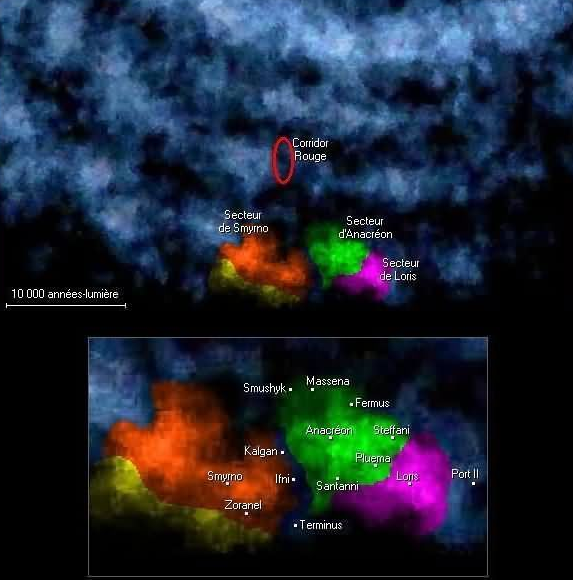
\includegraphics[width=10cm]{galactographie.png}
\end{center}
}

\paragraph{Synopsis}
{
Le gouverneur d’\textsc{Anacréon} et plusieurs de ses conseillers reçoivent l’inspection d’un homme de l’Empire (venant de \textsc{Trantor}).
Le vaisseau impérial a atteri sur la lune habitée d’\textsc{Anacréon}, où il a été accueilli l’ambassadeur.  Il se dirige à présent vers la planête principale.
}

\newpage

\mj{
\section{Présentation globale des personnages}

\paragraph{Paul \textsc{Ledar}}
{
Le gouverneur d’\textsc{Anacréon}.
Il détourne des montagnes d’argent qu’il utilise en grande partie en dessous de table pour se faire renommer gouverneur tous les quatre ans.
}

\paragraph{Leopold \textsc{Ledar} (fusion avec Paul \textsc{Ledar})}
{
Le fils du gouverneur, qui aimerait bien avoir le pouvoir un jour.
Son pouvoir politique n’est pas forcément si important, mais la pression de son père sur la planète le fait croire très influent.
Il est officiellement parmi les conseillers du gouverneur (même si ce n’est pas de lui que sortira la moindre idée constructive) et c’est lui le préfet de \textsc{Meneleus}.
La seule chose dont il est courant pour les disparitions sur \textsc{Meneleus}, c’est que l’hypothèse d’un trafic d’armes et de soldats pour aller combattre sur \textsc{Ifni}, une planète du secteur voisin \textsc{Smyrno}, semble la plus probable vu les affrontements qu’il s’y produit actuellement (bien que le gouvernement de \textsc{Smyrno} tente d’étouffer au maximum l’affaire ; \textsc{Trantor} ne sait d’ailleurs absolument rien de tout cela\ldots).
L’autre piste possible est que ce soit la rébellion qui ait installé sa base ici et qui recrute activement.
}

\paragraph{Dan \textsc{Sonen}}
{
Un des conseillers du gouverneur.
C’est en réalité un robot réactivé au tout début de l’empire par un Spacer extrémiste.
Il n’a pas vraiment réfléchit pendant ses millénaires d’existence à une quelconque loi zéro.
Il cherche à tout moment à ne pas laisser paraître le moindre indice de sa non humanité.
Son but est de faire respecter les lois (il n’en invente que très peu), quelque soit l’absurdité de celles-ci (du moment que l’on ne parle pas de tuer directement des êtres humains).
C’est ainsi que, bien qu’ayant suffisamment de détails pour savoir que Paul \textsc{Ledar} détourne de l’argent pour se faire réélire, il ignore tout simplement cela~: ce n’est pas à lui de s’en occuper.
Mais lorsqu’il y réfléchit un peu plus, le côté légal de toute cette affaire semble pour le moins douteuse.
Il a entendu parler des réseaux de drogue à \textsc{Anacréon} et c’est l’affaire sur lequel il réfléchit activement actuellement.
}

\paragraph{Bran \textsc{Colek}}
{
Un autre conseiller du gouverneur.
Celui-ci est beaucoup moins honnête et est le meneur principal d’un réseau d’esclavage (ces derniers sont enlevés à \textsc{Meneleus}) et de drogues (sur \textsc{Anacréon}).
Autant que possible, s’il pouvait étouffer les rumeurs venant de \textsc{Meneleus}, il le fera.
Il n’a jamais hésité à assassiner (jamais directement) des personnes qui en savaient trop.
Il profite beaucoup que Paul \textsc{Ledar} soit suffisamment naïf.
Il préfère par contre largement être celui qui tire les ficelles dans l’ombre à devenir gouverneur.
}

\paragraph{Vad \textsc{Shyvo}}
{
C’est l’inspecteur.
S’il a choisi cette mission, c’est bien parce qu’il a à faire dans les environs.
Il connaît en effet l’existence du réseau d’esclavage de Briran \textsc{Corllek} en tant que\ldots client.
Il compte bien rentabiliser une petite planète inhabitée (car trop froide) contenant d’après les scanners de nombreux minerais précieux.
Il est donc favorable à ce petit «~commerce~» et empêchera quiconque fera mine de vouloir l’enlever.
Mais les affaires deviennent compliquées puisque les «~incidents~» sur \textsc{Meneleus} commencent à se faire connaître.
Il veut éviter à tout pris de devoir mettre ceci sur son rapport — à moins bien sûr que l’on trouve un faux coupable à arrêter.
On lui a de plus collé un fonctionnaire qui fouine un peu trop et il aimerait trouver moyen de s’en débarrasser.
}

\paragraph{Nurn \textsc{Hazon}}
{
Le «~compagnon~» de l’inspecteur.
Il a été envoyé par l’administration de \textsc{Trantor} sous la pression (discrète néanmoins) de nombreux rivaux de Vad \textsc{Shyvo}.
Il a comme mission officielle d’aider l’inspection, mais comme mission officieuse de trouver le plus possible d’éléments pouvant décrédibiliser \textsc{Shyvo}.
Il a actuellement besoin d’argent, et c’est la principale raison pour laquelle il a accepté la mission~: il est devenu de plus en plus dépendant de drogues exotiques, et le fait de devoir se projeter en province ne l’enchante pas tellement. C’est un drogué, certes, mais pas régulier~: il a des vagues d’humeurs, ses «~périodes~».
Si seulement il pouvait trouver une petite friandise locale pour se soulager un petit peu.
}

\paragraph{Plaïa \textsc{Idaski}}
{
C’est elle le chef de la sécurité.
Elle sympathise avec le groupe de résistance d’\textsc{Anacréon} contre le gouverneur toujours réélu dont les soupçons de détournement d’argent découverts commencent à devenir trop nombreux.
Cependant, elle ne veut en aucun cas perdre sa vie, ou la passer en prison pour le reste du temps.
Elle fera ce qu’elle peut pour qu’aucune confrontation se passe lors du transport (les caméras sont partout dans ce vaisseau, mais la plupart sont retransmises directement au centrale sur la planète mère).
Mais elle ne fera rien pour emprisonner les résistants du vaisseau, elle est d’ailleurs au courant pour le responsable des communications.
Elle doit briefer au tout début du jeu Dacan \textsc{Calrines}, qui semble étrange aujourd’hui.
}

\paragraph{Nuv \textsc{Harset}}
{
Le responsable des communications.
C’est un agent de la résistance locale assez engagé~: il n’hésitera pas une seconde à mettre sa vie en danger si cela peut permettre de rétablir une démocratie ou quelque chose de ressemblant sur \textsc{Anacréon}.
Deux types de communications vont transiter~: celles de la résistance et les autres.
La plupart des machines sont automatisées, il s’occupe juste de faire l’interface avec le reste du vaisseau (il a une puce électronique dans l’oreille qui lui indique du nouveau, ce qui lui permet de se déplacer librement dans le vaisseau).
Il apprendra au cours de la partie que parmi les personnes présentes sur le vaisseau, au moins l’une d’elle fait des affaires à \textsc{Anacréon} avec les réseaux de drogue ; découvrir son identité sera très utile à la rébellion, puis une fois découverte, l’éliminer pourra être un objectif (tout dépend si la rébellion pourra se servir de l’information).
Puis rebellotte, mais pour des affaires à \textsc{Meneleus} (la rébellion ne sait pas exactement de quoi il s’agit).
}

\paragraph{Denik \textsc{Calkor} (fusion avec Nuv \textsc{Harset})}
{
Garde du corps de Paul \textsc{Ledar}.
Ce qui l’intéresse, c’est l’argent, les médailles à mettre sur son bel uniforme et tout les avantages que l’on pourrait imaginer.
Extérieurement, il semble pourtant incapable d’accepter la moindre condition qui le détournerait de sa mission.
Il porte un bon blaster et il est capable de menacer ou de tuer quelqu’un pour obtenir des informations sans hésiter.
On lui laisse toujours la possibilité d’aller voir le gouverneur (qu’il discute ou non avec un autre personnage important) et en connaît donc parfois long.
Il est censé obéir au gouverneur sans discuter. (Sauf si celui-ci lui demande de partir.)
Les personnes présentes sur le vaisseau ont l’air louches, et il aimerait en découvrir plus, puis — suivant le cas — en soutirer de l’argent contre la promesse de ne pas divulguer d’informations, ou les éliminer (d’une manière ou d’une autre~: on peut tout simplement les dénoncer parfois\ldots).
Il est un client assez régulier du réseau de drogue locale, heureusement que personne ne penserait à faire des tests très poussés sur sa personne (ce serait plutôt à lui d’exiger de quelqu’un un tel contrôle.).
Dacan \textsc{Calrines} semble avoir un petit stocke chez lui, mais il n’est en pas sûr.
Il va chercher à faire affaire avec.
}

\paragraph{Avalga \textsc{Orzon}}
{
Une très riche propriétaire d’\textsc{Anacréon}.
C’est aussi une amie politique du gouverneur.
Il y a déjà eu de nombreux échanges d’argent dans les deux sens entre eux (rarement légal).
Elle a déjà eu de nombreux problèmes avec la résistance, qui se doutait que les jugements étaient truqués.
Très intéressée par l’argent ou tout autre avantage, elle marchande tout ce qu’elle peut.
Elle va chercher à créer de nouveaux accords commerciaux avec les différents personnages importants du vaisseau, honnêtes ou non, du moment qu’ils rapportent.
Elle a entendue parler par exemple d’un trafic d’armes sur \textsc{Meneleus}, et ça l’intéresse grandement.
}

\paragraph{Yon \textsc{Bunki}}
{
Le médecin du vaisseau.
Il n’a jamais porté dans son cœur le gouverneur, mais il reçoit du fait de sa position tant de menaces sur sa famille qu’il ne fera pas grand chose qui risquerait de l’inculper.
Néanmoins, il sympathise avec la rébellion et fera tout ce qu’il peut pour les aider tant que sa famille ne risquera rien (c’est à dire que l’on ne puisse pas savoir qu’il est impliqué là dedans).
Il a découvert dans des toilettes collectives une poudre qu’il a analysé comme étant de la drogue similaire à celle du trafic sur \textsc{Anacréon}.
Il ne dira rien à personne sans savoir qui ici est un drogué, mais ce genre d’informations peuvent être très utiles.
}

\paragraph{Yanri \textsc{Trader}}
{
Espionne du secteur d’à côté, \textsc{Smyrno} (originaire de la planète principale, \textsc{Smyrno}).
Elle cherche à enquêter sur le gouverneur et les différentes magouilles qu’il s’y passe par ici.
Elle connaît la rébellion de réputation et aimerait se faire connaître en tant qu’allié d’eux (oui, elle joue triple jeu).
Son but est de faire couler le secteur d’\textsc{Anacréon} et fera tout pour que la situation politique ici soit le plus instable possible.
C’est elle qui a remplacé les pilules contre la toux de Dacan \textsc{Calrines}, la seule personne un peu honnête ici, par des pilules mnémoniques et a convaincu plusieurs personnes (en laissant des indices, pas en leur disant) qu’il ferait un trafic d’armes dans la région de \textsc{Meneleus}.
Elle se fait passer pour la responsable technique, ce qui lui a permis d’infiltrer quelques mouchard qui pourront être récupérés pendant la partie.
Personne ne lui fera la moindre remarque sur son travail~: c’est quasiment la seule ici qui s’y connaît un minimum en technologie.
}

\paragraph{Dacan \textsc{Calrines} (supprimé)}
{
Il ne se rappelle même pas de son nom, à par en lisant la plaque inscrite sur son uniforme.
En fouillant dans ses affaires, il a découvert une caisse de blaster (déposée par Vanri \textsc{Thrawder}), mais il n’en sait rien, ainsi qu’un tas non négligeable de crédits.
Parmi les documents qu’il lit, il semblerait qu’il soit à la tête d’un trafic d’armes sur \textsc{Meneleus}.
Bien entendu, rien ne lui revient en mémoire.
Il remarque un mot de lui dans sa chambre~: il a rendez-vous avec Plaïa \textsc{Idaski} pour un briefing de la mission actuelle.
Avant que Vanri \textsc{Thrawder} mette le désordre dans sa tête, il était juste un agent de sécurité aux ordre de Plaïa \textsc{Idaski}.
Pas des plus finaux, mais il faisait toujours bien son travail.
Il était un des nombreux «~terminaux~» du trafic de drogue.
Il n’a jamais fait de nombreuses affaires, mais il a acheté des quantités relativement grandes de drogue (pour une dizaine de personnes), qu’il comptait revendre à \textsc{Anacréon}.
Cette drogue est cachée dans un oreiller, et il l’a repéré lors de ses fouilles.
Par contre, il ne voit pas du tout ce que ça peut bien être\ldots
}

\newpage
}

\mj{
\section{Possessions initiales des personnages}

\begin{center}
\begin{tabular}{|c|c|c|c|c|}
\hline Personnage & Argent initial & 250 & 500 & 1~000 \\
\hline\hline
Paul \textsc{Ledar} & 5~500 & 0 & 3 & 4 \\
\hline
Dan \textsc{Sonen} & 1~250 & 1 & 2 & 0 \\
\hline
Bran \textsc{Colek} & 6~500 & 2 & 4 & 4 \\
\hline
Vad \textsc{Shyvo} & 2~000 & 0 & 0 & 2 \\
\hline
Nurn \textsc{Hazon} & 3~000 & 2 & 3 & 1 \\
\hline
Plaïa \textsc{Idaski} & 1~000 & 2 & 1 & 0 \\
\hline
Nuv \textsc{Harset} & 1~250 & 3 & 1 & 0 \\
\hline
Avalga \textsc{Orzon} & 5~500 & 0 & 1 & 5 \\
\hline
Yon \textsc{Bunki} & 1~750 & 3 & 2 & 0 \\
\hline
Yanri \textsc{Trader} & 3~750 & 5 & 1 & 2 \\
\hline
\end{tabular}
\end{center}
}

\mj{
\section{Fin possibles}

\begin{itemize}
	\item \textsc{Anacréon} déclare l’indépendance à l’Empire.
	\item La Rébellion a suffisamment d’informations pour préparer un coup d’état à l’arrivée du vaisseau~:  Paul \textsc{Ledar} fini assassiné.
	\item Le gouvernement arrive à contrer ce coup d’état.
	\item \textsc{Trantor} retire le poste de gouverneur à Paul \textsc{Ledar}.
\end{itemize}
}

\mj{
\section{Événements}

\begin{itemize}
\item Avalga ou Ledar apprend qu’un espion de Smyrno est vraisemblablement dans le vaisseau — un message ayant été capté puis décrypté par hasard depuis une des stations qu’ils contrôlent.
\item Le médecin apprend que sa famille a été massacrée.
\item Ledar apprend qu’il y a des rebelles dans le vaisseau.
\item Ledar apprends qu’un de son conseiller est peut-être mêlé à des histoires d’esclavages sur Meneleus.
\item Le médecin découvre que le robot vient de faire un mouvement qui d’ordinaire n’est pas possible pour un humain.
\item L’ambassadeur reçoit un ordre de Trantor de destitution temporaire du gouverneur : trop de doutes portent sur lui sur de vieilles affaires et l’administration de la planète préfère le remplacer par un de ces conseillers le temps qu’il s’explique.
\item Ordre d’une partie de l’administration de Trantor pour le fonctionnaire : déclenchez un scandale immédiatement contre l’ambassadeur, cela devient trop urgent.
\item Idaski aperçoit une action de quelqu’un qui peut permettre de l’aider sensiblement à mettre le bazar.
\item L’ancien résistant (le médecin donc) reçoit comme ordre de se faire d’une alliée/tuer Avalga.
\item Nuv Harset apprend que l’une des personnes du vaisseau est impliquée dans les réseaux de drogue sur Anacréon.
\item Quelqu’un (l’espionne ou le secrétaire) découvre que c’est le conseiller véreux qui a fait assassiner la femme de Paul Ledar.
\end{itemize}
}

\mj{\newpage}

\player{1}{
\section{Ton personnage~: Paul \textsc{Ledar}}

\paragraph{Description physique}
{
	Pas spécialement grand, en dessous de la moyenne anacréonnienne.
	Il est cependant très bien habillé (c’est le gouverneur).

	Il possède 5~500 crédits initialement, mais il en possède bien plus sur \textsc{Anacréon}.  Disons que ces crédits sont juste ce qu’il faut pour servir d’engagement à des dessous de tables (tant que l’on promet que la personne recevra le triple à l’arrivée).
}

\paragraph{Ton personnage}
{
Toi au moins, tu as bien compris ce que c’était que la politique~!
La politique, c’est ta vie. Jamais tu ne laisseras quelqu’un te marcher sur les pieds, même si cela t’a parfois coûté très cher.
Peu après ton arrivée au pouvoir, on t’a fait savoir que le peuple était fermement opposé à tes directives.  Pourtant, et contre l’avis contraire de ton conseiller Bran \textsc{Colek}, tu as insisté dans ta politique.
En réponse, ta femme — plus vulnérable que toi-même — a été prise pour cible lors d’un attentat d’opposants à ton régime.  Depuis tu ne te laisses toujours pas marcher sur les pieds, mais tu utilises des méthodes plus… subtiles.  Tes conseillers t’aident grandement en cela.

Cela va bientôt faire dix ans que tu occupes ce poste de gouverneur d’\textsc{Anacréon}.
Gouverneur, c’est une bonne position, surtout d’un système aussi éloigné du centre de la Galaxie, \textsc{Trantor}.
Habituellement, un gouverneur est réélu tous les quatre ans. Mais bon… Les dessous de tables ont toujours existé.
Et tu n’as aucune intention de lâcher ce poste.

Tu as déjà envisagé de supprimer cette loi qui fait apparaître un semblant de démocratie à ta dictature, mais jamais le peuple anacréonnien n’acceptera cela.
Cela t’embêtes beaucoup d’ailleurs car cela te coûtes de plus en plus cher.
Certes, tu détournes plus d’argent que tu en utilises pour te faire élire, mais ça t’embête tout de même.

Heureusement qu’il y a ton garde du corps Nuv \textsc{Harset}.
Ce serait un suicide de s’en débarrasser plus d’un quart d’heure, surtout par les temps qui court.
Un grand gars qui t’obéit au doigt et à l’œil, c’est toujours pratique.
Il s’occupe de plus des diverses communications et te sert de secrétaire à ses heures.

Tu connais bien Avalga \textsc{Orzon}, c’est une riche propriétaire avec qui tu as souvent fait affaire.
Il serrait de bon goût pour toi de conclure une nouvelle affaire ici~:  si ne serais ce que la moitié de ses relations étaient à ton service pour truquer les élections, ce serait tellement plus simple.
Il faudrait lui donner quelques terres sur une planète du système, peut-être cela suffirait.

Peut-être \textsc{Meneleus}~?
C’est certes une grande planète, mais a le désavantage d’être complètement gelée (pourtant ses habitant semblent le supporter), non, ce n’est pas l’idéal ; surtout que des rumeurs diraient que la rébellion aurait fondé des avant-postes sur cette planète…
D’ailleurs, depuis cette fichu rébellion, ton électorat ne cesse de descendre~!
Il faudrait que tu demandes un peu d’aide à tes fidèles conseillers Dan \textsc{Sonen} et Bran \textsc{Colek}, qui sont assez bon dans leur métier, il faut le dire.

Le vaisseau est assez grand et tu ne connais pas tout le monde.
Serait-ce possible que des rebelles se cachent ici même~?
Non, ils auraient dus passer les sécurités, et Plaïa \textsc{Idaski} est assez ferme sur ce genre de points.
De toute façon, tu as ton garde du corps.

Ce vaisseau est actuellement en route pour \textsc{Anacréon}, la planète principale du système.
Il vient d’accueillir l’ambassadeur de l’Empire.
Ça, c’est vraiment ton plus gros problème actuellement.
Tu sais très bien que tout ne se passe pas très bien dans le système, et tu n’as aucune envie de devoir faire un rapport à un représentant de \textsc{Trantor}.
Mais bon, il n’y a aucune solution~: on ne va pas chercher des ennuis avec l’Empire.

Par contre, cela ne veut pas dire du tout que tu vas leur annoncer la vérité sur un plateau.
Non, il va falloir improviser, mais il est hors de question que \textsc{Trantor} se doute de quoi que ce soit sur ce qui ce passe exactement ici.
}

\paragraph{Objectifs}{
\begin{itemize}
	\item Empêcher tout mauvais rapport à \textsc{Trantor} afin de garder sa place.
	\item Obtenir de nouveaux «~traités~» officieux pour t’aider à garder t place de gouverneur.
	\item Tenter d’obtenir de nouvelles informations sur la rébellion.
\end{itemize}
}
}

\player{2}{
\section{Ton personnage~: Dan \textsc{Sonen}}

Ton personnage est en réalité un robot~:
avant l’Empire, il y avait deux «~clans~» — les \textit{Spacers} et les \textit{Settlers}.
Pour faire vite~: les \textsc{Spacers} vivaient sur une dizaine de planètes, pouvaient vivre jusqu’à plusieurs centaines d’années, et vivaient au milieu d’une foule de robot dans une société où le taux de natalité était contrôlé afin d’éviter toute surpopulation. Ils avaient eu pendant très longtemps le contrôle politique de la Terre.
Les \textsc{Settlers} quant à eux sont d’anciens terriens qui ont réussi à se libérer de l’hégémonie des \textsc{Spacers}. Ils refusaient tous robots, et ont permis de rapidement construire ce que l’on appelle maintenant l’«~Empire~».

Ces histoires ont maintenant été complètement oubliées de la part des hommes (jusqu’à leur planète d’origine et la notion «~d’avant l’Empire~», qui leur est devenue étrangère).

Tu as été réactivé bien après la fin de l’hégémonie \textsc{Spacer} par un extrémiste voulant redonner une chance aux robots.
Comme tout robot, tu suis les trois lois de la robotique~:
\begin{itemize}
	\item Jamais tu ne feras du mal à un humain, que se soit en faisant une action ou en ne faisant pas une action.
	\item Tant que les ordres des autres humains ne contredisent pas la règle précédente, tu obéis aveuglement aux humains.
	\item Tant que tu ne désobéis pas aux deux lois précédentes, tu tentes autant que tu peux de te protéger toi-même.
\end{itemize}
Autant la première loi n’est pas très complexe à comprendre, autant la seconde cache de très nombreux cas particuliers~:  que se passe-t-il par exemple si deux humains te donnent deux ordres contradictoires~?
En cas de toute sur la seconde loi, il faut savoir que comparée à toute ta perfection de conception et ta complexité de raisonnement, les circuits qui interprètent la seconde loi sont relativement simplistes et s’appuient sur une interprétation sémantique de la phrase.
Typiquement, si l’on te demande «~Pouvez-vous faire quelque chose~?~», tu n’es pas forcé de voir cela comme un ordre.  Bien entendu, si l’on te demande de faire quelque chose, c’en est clairement un.
De plus tu as remarqué que la plupart des ordres donnés par les humains sont laissés à interprétations, et qu’il est souvent possible de réaliser une «~variante~» de l’ordre.  Par exemple, l’ordre «~Faites en sorte que~» peut très bien être accompli en demandant à quelqu’un de le faire à ta place.
Dans tous les cas, n’oublie pas que la première loi prime de toute façon, et aussi que les hommes ont maintenant peur des robots~:  la troisième loi va donc t’obliger à empêcher les autres de découvrir que tu es un robot.
Ce n’est pas parce que tu dois obéir aux ordres des humains que tu ne peux pas t’arranger pour que les humains ne te donnent pas d’ordre~!

D’apparence extérieure, tu ressembles totalement à un humain, aux différences près que tu as tendance à paraître sans émotion la plupart tout le temps.
Par contre, comme tout robot, tu as une force extraordinaire.  (Mais tu ne la montre jamais, sauf si cela contredit les deux premières lois pour éviter que l’on te prenne pour un robot…)
Contrairement à Daneel \textsc{Olivaw}\footnote{Si tu connais l’univers…  Sinon, tu peux tout simplement ignorer cette remarque.}, tu n’a jamais vraiment réfléchi à la possibilité d’une «~loi zéro~».

En tant que robot, tu as bien vu que si tu restais à \textsc{Trantor}, le centre de l’Empire, jamais tu ne pourrais éviter d’être repéré comme étant un robot (ne serais-ce que parce que tu ne vieilli pas).
Tu as donc décidé (suivant la troisième loi) de partir dans les périphéries de la Galaxie.

Cela va bientôt faire près de 13~000~ans que tu as été activé.
Depuis ce temps là, tu est passé de systèmes en systèmes dans les périphéries de la Galaxie.
Tu te fais passer pour un humain, tu tentes de te faire le moins remarquer possible, tout en prenant part à la vie humaine.
Assez souvent, tu restes environ 60~ans sur une planète avant de changer de système.

Cette fois-ci, il semble que tu ais été particulièrement chanceux~:
En arrivant sur \textsc{Anacréon}, tu t’es très vite fait repéré en sauvant un habitant.
Tu t’es assez vite lié d’amitié avec lui.  (Depuis le temps, tu as l’habitude de parler sans jamais te trahir.)
Ta capacité à calculer des probabilités d’actions ou de décision c’est assez vite trouvée utile ici~:  tu as réussi à te faire nommer conseiller du gouverneur.
Ceci te permet de posséder un pouvoir suffisant pour éviter tout test médical sur ta personne (qui pourrait avoir de mauvaises conséquences pour toi…) tout en restant plus ou moins dans l’ombre médiatique du secteur.

Comme tout robot, ton idée de la «~Justice~» est assez simpliste~:  elle consiste à suivre les lois (de la robotique, comme les lois humaines).
Inventer une loi n’est ainsi pas ton fort, sauf si cela renforce une autre.
Souvent, tu te contentes d’indiquer au gouverneur Paul \textsc{Ledar} ce que tu considères comme étant l’action politique la plus probable~:  tes processeurs sont en effet extrêmement efficaces pour déterminer la réaction d’un grand nombre d’humains à une action donnée.

Tu as déjà eu suffisamment d’indices pour voir que Paul \textsc{Ledar} détournait des quantités d’argent dans le seul but de se faire réélire.
Tu trouves cela assez louche, mais comme ces lois sont (pour toi) ambigües, tu ne vois vraiment le problème.
En fin de compte, tu ignores simplement cette affaire, même si tu pourrais possiblement l’exprimer sans y penser.

Tu sais très bien ce qui pourrais se passer si on te donnait un ordre~: tu le suivrais sans même réfléchir.
Pour éviter cela, tu as appris à ne jamais te mêler d’affaires qui ne te concerne pas, à rester proche de Paul \textsc{Ledar}, où jamais personne n’oserait te donner un ordre direct.  (Tu es tout de même le conseiller du gouverneur~!)
Depuis le temps que tu es activé, tu as su trouver des «~limites~» aux lois robotiques~:  par exemple si quelqu’un te demande ce que tu sais sur tel sujet, il ne te demande pas directement de dire tout ce que tu sais, mais juste de dire ce que tu penses \emph{pourrais} être vrai compte-tenu de tes informations par exemple.
Tu as su jouer sur ce tranchant de la langue pendant un certain temps.

Actuellement, ton rôle de conseiller est de mettre au clair ce qui se passe exactement à \textsc{Anacréon} concernant les trafics de drogue.
Pour l’instant, la seule chose que tu sais dessus est la présence de quelques réseaux.
En soupesant les probabilités, tu penses que la majeur partie se trouve dans la ville de \textsc{Concatalle}, mais tu n’en sais pas encore assez pour pouvoir effectuer la moindre action de la part du gouvernement.

\paragraph{Capacités spéciales}
{
Ton personnage possède une force surhumaine.
Il a aussi une très grande connaissance d’énormément d’affaires louches dans la Galaxie.

Bien entendu, il ne va pas le montrer à tout le monde, de peur de montrer aux autres sa véritable identité ; mais s’il se produit un cas où il se retrouve avoir besoin de le faire (par exemple pour obéir à une des lois), merci d’appeler un maître du jeu.
}

Tu possèdes initialement 1~250 crédits.
Tu ne sais pas vraiment ce que cela vaut, mais quelqu’un avec qui tu as discuté il y a plusieurs centaines d’années t’as dit de toujours avoir de l’argent sur toi (il t’a dit à l’époque que ça pouvait toujours servir).
Sa formulation avait alors activé la seconde loi et tu ne peux pas vraiment lui désobéir, même après tout ce temps.

\paragraph{Objectifs}{
\begin{itemize}
	\item Respecter les trois lois de la robotique.
	\item Éviter que quelqu’un découvre que tu es en réalité un robot.
	\item Trouver le plus possible d’informations sur les trafics de drogue du système (et faire appliquer des lois de répression des trafics si cela est possible).
\end{itemize}
}
}

\player{3}{
\section{Ton personnage~: Bran \textsc{Colek}}

Dans ta vie, tu as très rapidement compris ceci~:
les gens sont faibles et facilement manipulables à ta volonté.
Beaucoup sont cupides et une simple somme d’argent peut suffire à les faire changer d’avis, de parti politique ou même à les faire oublier quelque chose.

Depuis que tu as compris ceci, rien ne t’arrête.
Tu sais manipuler les lois de façon à leur faire dire ce que tu veux, tu n’as jamais hésité à soudoyer, menacer, torturer ou faire tuer pour arriver à tes fins.

Tu es relativement rapidement devenu un des meneurs principaux des réseaux d’esclavage et de drogue du secteur.
Le réseau d’esclavage est un réseau enlevant des travailleurs sur une petite planète froide du secteur, \textsc{Meneleus}, pour les exporter dans d’autres secteurs de la Galaxie.
Quant au réseau de drogue, tout se passe sur \textsc{Anacréon}.
La drogue locale est une poudre brunâtre qui se vend assez cher.

Bien entendu, rien de tout cela n’est légal, mais bon, pourquoi suivre les lois si cela reviendrait à perdre une partie de ses pouvoirs~?
Tu n’es pas un de ces faibles~!

Tu as de plus réussi à avoir une des meilleurs positions auxquelles tu pouvais espérer~:
Tu es un des conseillers du gouverneur Paul \textsc{Ledar}.
Paul \textsc{Ledar}, l’exemple typique d’un humain \textit{faible}.
Il suit quasiment tous tes «~conseil~» à la lettre — bien entendu, tu fais tout ce qu’il est de ton possible pour que ces conseils paraissent à son avantage.
Cela est d’autant plus facile que l’unique fois où il t’a fermement désapprouvé, tu as fait assassiner sa femme en mettant ce meurtre au compte d’une réponse du peuple à sa politique.

Tu as vite découvert que suivre les lois n’était pas non plus dans ses objectifs, et tu l’as fait lancer une grande campagne de dessous de table pour rester au pouvoir.
Comme s’il était le premier~!
Ce qui est rigolo avec lui, c’est qu’il a des… remords.
Quel faible~!

En pratique, tu es donc la personne qui tire les ficelles derrière l’ombre, qui contrôle tout le gouvernement d’\textsc{Anacréon}.
Ça te va très bien.

Bien entendu, il est déjà arrivé de nombreux cas où il n’a pas suivi tes conseils.
Il l’a vite regretté~: à chaque fois, tu faisais assassiner un de ses proches et faisait passer cet assassinat comme une réponse du peuple à son inaction.
Et il te croit~!

Il y a actuellement quelques rumeurs venant de \textsc{Meneleus} à propos de ton trafic d’esclaves.
Si seulement tu pouvais les étouffer.

Il y a de plus cet envoyé de \textsc{Trantor} qui peut tout gâcher.
Quels fouineurs à \textsc{Trantor}, comme s’ils avaient encore du pouvoir ici~!
Comment vas-tu faire pour t’en débarrasser~?

\paragraph{Compétences spéciales}
{
Tu connais très bien les réseaux d’assassinat d’\textsc{Anacréon}, et vous avez des «~codes~» qui vous permettront de communiquer sans que personne ne comprennent.
Si tu souhaites faire assassiner un proche de quelqu’un dans ce vaisseau (voire un des membres du vaisseau~!), tu n’as qu’à prévenir un des maîtres du jeu.
(Attention, l’assassinat pourra prendre quelques temps avant d’avoir effectivement lieu~!)
}

Tu possèdes sur toi quelques 6~500 crédits.
Cela n’est pas si énorme, mais cela est parfait pour servir de garantie (tant que tu promets le quadruple à l’arrivée du vaisseau sur la planète) pour un «~accord~» illégal.

\paragraph{Objectifs}{
\begin{itemize}
	\item Se débarrasser \textit{discrètement} des gêneurs trantoriens.
	\item Étouffer toute rumeur provenant de ton trafic d’esclaves (par exemple en lançant d’autres rumeurs).
	\item Garder ton contrôle sur le gouverneur (entre autres, il doit ignorer que tu le manipules).
	\item Si possible, passer quelques nouveaux accords afin de commencer de nouveaux trafics.
\end{itemize}
}
}

\player{4}{
\section{Ton personnage~: Vad \textsc{Shyvo}}

Tu viens de la planète \textsc{Trantor}, le centre administratif de l’Empire Galactique.
Pourquoi te retrouver ainsi perdu au milieu d’un secteur de la périphérie de la Galaxie~?
C’est une longue histoire en fait…

Officiellement, tu es fonctionnaire de \textsc{Trantor}, mais en réalité, ta principale «~cible~» actuelle n’est pas ces paperasses de fonctionnaires, non.
Tu as récemment «~acheté~»\footnote{
Il va sans dire qu’«~acheter~» est synonyme ici de dessous de table, de corruption, etc.
} le monopole d’une planète relativement récemment découverte (il y a une dizaine d’années).

Cette planète totalement inhabitée (car beaucoup trop froide) contiendrait d’après les scanners de nombreux stocks de minerais précieux.
Tu cherches donc de la main d’œuvre pas cher capable de s’adapter à une telle planète.

Et une telle main d’œuvre, tu sais où en trouver ici.
En effet, tu connais de sources à peu près fiables qu’un certain Bran \textsc{Colek} organise un trafic d’esclaves venant d’une planète froide nommée \textsc{Mélènus}, ou quelque chose comme ça.
Cette personne a l’air d’avoir pas mal d’antécédents~: tu es sûr de pouvoir faire affaire avec.

C’est la raison principale pour laquelle tu as accepté cette mission d’inspection.
Ta mission officielle est de faire un rapport exact sur ce qui se passe dans la périphérie, en particulier tout ce qui pourrait coller avec toute contradiction avec les lois officielles de \textsc{Trantor}.

Bien entendu, il serait de bon ton pour tes affaires de ne pas mettre par écrit cette histoire d’esclavage…  À moins bien sûr de trouver des «~preuves~» contre un faux coupable qui serait arrêté par le gouverneur local, Paul \textsc{Ledar}.
Il faudrait aussi conclure ce pacte avec ce \textsc{Colek}.
Tu as vraiment besoin de ses esclaves.

Ah oui, il reste un petit détail.
On t’a collé un fonctionnaire pour t’assister dans ta mission officielle et celui-ci a une fâcheuse tendance à fouiner un peu partout — un peu trop aussi.
Si seulement tu pouvais t’en débarrasser… Ça te simplifierait de beaucoup la tâche~: s’il en venait à découvrir cette histoire de trafic d’esclaves, tu serrais forcé de le mettre sur ton rapport, ce qui détruira toutes tes espérances d’exploitations minières.

Tu possèdes environ 2~000 crédits.
Tu ne sais pas combien de temps cela te permettrais de vivre ici, mais à \textsc{Trantor}, cela est l’équivalent de deux ou trois mois de salaire d’un fonctionnaire\footnote{En sachant que les prix en campagne ont la réputation d’être ridicules par rapport à ceux du centre.}.

\paragraph{Objectifs}{
\begin{itemize}
	\item Conclure un accord pour un trafic d’esclave.
	\item Ne pas écrire sur le rapport la moindre chose qui pourrait faire suspecter l’existence d’un tel trafic dans le système.  Cela implique de surveiller ou d’éliminer le fonctionnaire Nurn \textsc{Hazon}.
\end{itemize}
}
}

\player{5}{
\section{Ton personnage~: Nurn \textsc{Hazon}}

Tu viens de la planète \textsc{Trantor}.
Tu y occupes un rôle de fonctionnaire de l’administration de la Capitale Impériale.
Si tu es ici, c’est officiellement pour assister Vad \textsc{Shyvo} dans une mission ; ce dernier doit en effet faire une mission de reconnaissance dans le secteur d’\textsc{Anacréon}, il paraîtrait que des choses louches s’y passent.
C’est une région de la périphérie de la Galaxie qui semble perdre un peu les derniers fondements de démocratie qui s’y appliquait.
Bon, ça, tu t’en fiches.  Que ces hommes qui ne respectent pas les lois de l’Empire se débrouillent comme ils veulent, du moment qu’ils ne se rapproche pas du centre.
(Mais ça, tu n’y crois juste pas~:  qui oserait affronter l’Empire de nos jours~?)

La vraie raison de ta présence est toute autre.
Vad \textsc{Shyvo} dérange pas mal les affaires de l’administration trantorienne, et plusieurs de ses opposants montrent une vive insistance pour qu’il soit… mis hors d’état de nuire les rouages de la précieuse administration de \textsc{Trantor}.
Cette pression est certes discrète, elle reste perceptible, et tu as réussi à négocier le prix fort à l’un de ses rivaux pour que tu l’accompagnes jusqu’ici.

C’est assez dangereux~:  tu pourrais y perdre ton poste à \textsc{Trantor} si tu te fait prendre.
Mais cela ne devrais pas arriver, tu sais faire les choses subtilement.
Il te faut trouver tout ce qui pourrait nuire ou décrédibiliser \textsc{Shyvo} à \textsc{Trantor}.
Tout peut servir.
Tu as pour cette mission acheté un petit appareil photographique.
Chaque photo «~intéressante~» peut te rapporter très gros.

La grande difficulté de ta mission consiste à constamment surveiller \textsc{Shyvo}, tout en lui faisant croire que tu t’intéresses à autre chose, afin qu’il puisse effectivement faire des erreurs diplomatiques sans qu’il ne se croit surveillé.
Il va aussi falloir que tu arrives à monter de fausses rumeurs contre lui~:  une photo d’un responsable de la sécurité le fouillant fera du plus mauvais effet à la Capitale~!

La raison pour laquelle tu as besoin d’argent est toute autre.
Depuis un certains temps, tu te drogues régulièrement.
Certes, pas toujours, tu as tes «~périodes~».
Ce que tu préfères, ce sont les drogues «~exotiques~».

Certes, d’un point de vue politique, la périphérie de la Galaxie est tout sauf intéressante, d’un point de vue «~exotique~», elle regorge de surprise.
L’importation coûte cher, surtout pour ce type de marchandises.
Si seulement tu pouvais profiter du séjour pour obtenir quelques petites «~friandises~» locales, ça te soulagerait peut-être.
D’ailleurs, tu étais sûr d’en avoir un peu sur toi, mais ton sachet est introuvable depuis que tu as embarqué sur ce vaisseau… où l’as tu donc égaré~?

\paragraph{Matériel}
{
Ton personnage possède un appareil photographique miniature caché dans son veston.

En cas d’utilisation, merci de prévenir un maître du jeu.

Tu possèdes 3~000 crédits, ce qui correspond à environ deux ans de salaire anacréonien moyen.
}

\paragraph{Objectifs}{
\begin{itemize}
	\item Trouver le plus d’éléments qui pourraient disculper l’ambassadeur Vad \textsc{Shyvo}.
	\item Si ces preuves ne sont pas suffisantes pour le disculper, s’arranger pour l’éliminer ici.
	\item Trouver et acheter (discrètement) des drogues locales.
	\item Ne pas te faire voir dans tes actions~:  tu ne tiens pas non plus à perdre ta place de fonctionnaire à \textsc{Trantor}.
\end{itemize}
}
}

\player{6}{
\section{Ton personnage~: Plaïa \textsc{Idaski}}

\paragraph{Description Physique}
{
Assez grande et costaude, genre garçon manqué.
}

Les détournements d’argent du gouverneur Paul \textsc{Ledar} commencent à bien faire, décidément, la résistance à raison~: il faut en finir avec son gouvernement de dessous de table et de corruption~!
Par contre, il faut le faire de manière subtile~:  l’idée même que tu pourrais y perdre la vie ou la passer en prison ne t’enchante guère…
Non, décidément, ce n’est pas toi qui tentera une quelconque action «~héroïque~» ou suicidaire contre lui.
Par contre, rien ne t’empêche d’aider des partisans ou des membres de la résistance si l’occasion se présentait.
À condition bien sûr que tu ne mettes pas tes mains là dedans~: hors de question de se faire prendre sur le vif~!

Tu penses d’ailleurs que tu va avoir quelques occasions lors de ce voyage.
En effet, c’est toi le chef de la sécurité du vaisseau menant le gouverneur vers la planète \textsc{Anacréon} ; il revient de la lune où il est allé souhaiter la bienvenue à un ambassadeur de \textsc{Trantor}, qui l’accompagne d’ailleurs actuellement.

Bon, tout ça ne te regarde pas.
Ce qui est important pour toi, c’est tout d’abord d’assurer la sécurité dans ce vaisseau.
Après, si l’occasion se présentait de pouvoir tuer le gouverneur ou renverser le gouvernement — et que tu ne risques absolument rien — tu feras probablement quelque chose.
Mais tu n’es pas encore là.
Pour l’instant, la sécurité du vaisseau d’abord.

Et puis de toute façon, que ferais-tu~?
Il y a des caméras partout dans le vaisseau, et la plupart retransmettent directement vers la planète mère.
Inutile de se faire des histoires~: si tu tires dans la direction du gouverneur, tout le monde saura que c’est toi une fois le vaisseau atterri.
Et tu ne le veux pour rien au monde.

Par contre, il pourrait être intéressant de voir ce que fera le secrétaire et soit-disant garde du corps du gouverneur, Nuv \textsc{Harset}.
En effet, tu as des raisons de croire que cet homme a un lien (probablement faible, mais présent) avec la résistance.
Après tout, s’il te «~vole~» ton blaster — ce qui t’empêchera de tirer dessus s’il tente quelque chose contre le gouverneur — comment pourrait-ce être de ta faute~?
Il reste à discuter discrètement avec lui pour voir ce qui se passe.
Remarque, en tant que chef de la sécurité, ça doit pouvoir s’arranger.

Certes cette position donne quelques avantages, mais elle donne aussi quelques responsabilités.
Tu connais les actions à faire en situation d’urgence par cœur, et ce sera à toi de les rappeler à tout le monde en cas de problème (qu’il soit dû à un évènement extérieur ou à un tué/blessé dans le vaisseau).
D’ailleurs, il est temps de vérifier que tout se passe bien~:  les passagers ont air de beaucoup discuter, cela peut vouloir dire beaucoup de choses…

\paragraph{Matériel}
{
Ton personnage possède un blaster.
Libre à toi de l’utiliser comme tu le souhaite, à condition de prévenir un maître du jeu à chaque utilisation.

Tu possède 1~000 crédits anacréonien, ce qui est l’équivalent de quasiment une année de ton salaire.
}

\paragraph{Objectifs}{
\begin{itemize}
	\item Assurer la sécurité du vaisseau.
	\item Tâcher d’assassiner le gouverneur à l’aide de membres de la résistance (s’il y en a dans le vaisseau), mais sans mettre ta propre vie en danger.
\end{itemize}
}
}

\player{7}{
\section{Ton personnage~: Nuv \textsc{Harset}}

\paragraph{Description physique}
{
Grand costaud.
Extérieurement, Nuv \textsc{Harset} a l’air totalement impassible et incorruptible.

Il possède sur lui une oreillette qui le relie au terminal de communication du vaisseau~:  c’est lui qui fait le lien entre le gouverneur et les communications externes du vaisseau.
}

\paragraph{Ton personnage}
{
Tu as toujours été convaincu que Paul \textsc{Ledar}, le gouverneur, est une crapule politique.
Il n’a jamais eu aucune conviction, jamais fait aucune action qui aurait permis d’aider la société du système.
Non, rien — par contre la corruption, ça il connaît bien.

Maintenant tu vois bien le système tel qu’il est~:  une dictature.
Certes, il y a encore des symboles (on offre un possible renouvellement du gouverneur — lorsqu’il n’est pas réélu), mais rien qui pourrait vraiment empêcher tout cela.

C’est donc tout naturellement que tu avais pris contact avec la Rébellion (ou plutôt que la Rébellion avait pris contact avec toi).
La Rébellion est un groupement secret principalement basé à l’époque à \textsc{Concatalle}, la ville où tu travaillais, qui vise à renverser le gouverneur pour rétablir une véritable démocratie.

Tu avais le profil physique parfait pour pouvoir un jour devenir le garde du corps d’une personnalité importante.
C’était ainsi en tant qu’agent de la Rébellion que tu t’es engagé dans les services de police dans le cadre de la protection d’officiels.
On t’a alors donné un entraînement incroyable, et tu es maintenant fier de faire partie de la garde personnelle du gouverneur.

Cependant, ces histoires de Rébellion, tu les as un peu oubliés.
Tu t’en rends compte maintenant~:  tu n’es pas fait pour faire le martyre ou le héros.
Il est hors de question pour toi de te suicider en abattant le gouverneur de tes propres mains.
Cela serait possible vu ta position bien entendu, mais tu te ferais abattre immédiatement par les autres policiers du coin.
De plus, il y a des caméras partout ici~:  même si tu arrives à en échapper, tu te feras rapidement juger puis condamner à mort.
Désolé pour la Rébellion, mais tu as échoué à la mission qu’ils t’avaient donnée.

Pourtant, tu ne les as pas encore informés de ton abandon~:  tu ne perds pas espoir qu’il y ait d’autres moyens moins dangereux pour rétablir la démocratie, et tu n’hésiteras pas à utiliser ta position pour le faire.
En plus d’être garde du corps du gouverneur, tu es en effet aussi son secrétaire~:  ton oreillette reçoit tous les messages venant de l’extérieur du vaisseau et c’est toi qui est censé les transmettre au gouverneur.
De plus, il a tendance à te faire relativement confiance~:  il vit tellement dans un monde de corruption qu’il en oublie que des gens comme toi peuvent agir~!
Ce sera donc un jeu d’enfant de modifier les messages qu’il reçoit à ton avantage.

Par contre, tu ne pourras probablement rien faire tout seul~:  il va falloir voir si tu as des alliés dans ce vaisseaux — mais pour cela il va falloir que tu t’éloignes du gouverneur afin de discuter avec eux ; malheureusement ce dernier refuse catégoriquement~!
Il doit y avoir un moyen de trouver une bonne excuse~:  si tu «~soupçonnes~» quelqu’un de vouloir attenter à la vie du gouverneur, celui-ci ne pourra probablement pas t’empêcher d’aller discuter avec lui (soit-disant pour l’en empêcher…).

Tiens~?  Ton oreillette sonne…
Une nouvelle importante~:  il semblerait que des disparitions régulières sur la planète \textsc{Meneleus} — une des planètes du système — se soient produites récemment.
L’hypothèse la plus probable serait un trafic d’armes et de soldats pour alimenter la guerre sur \textsc{Ifni}.
Il s’y produirait en effet ces temps-ci des affrontements assez belliqueux.
Mais tu n’en sais pas plus~:  le secteur de \textsc{Smyrno} où se trouve \textsc{Ifni} semble vouloir étouffer l’affaire.
Il paraît que même \textsc{Trantor} n’est pas au courant, c’est pour dire~!
Une autre hypothèse serait que la rébellion se soit installée sur la planète et qu’elle recrute activement.

À toi de choisir si tu annonces tout cela tel quel au gouverneur…
}

\paragraph{Matériel}
{
Nuv \textsc{Harset} possède une oreillette.
Lorsque le vaisseau reçoit une transmission de l’extérieur, les maîtres du jeu te préviendront.

Tu portes de plus sur toi un blaster.
Merci de prévenir les maîtres du jeu à chaque utilisation.

Tu possèdes 1~250 crédits.  C’est l’équivalent d’environ un an de ton salaire.
}

\paragraph{Objectifs}{
\begin{itemize}
	\item Voir si tu peux profiter de ton rapprochement du gouverneur pour pouvoir aider la Rébellion (en discréditant le gouverneur ou en détruisant ses alliances).
	\item Assurer la sécurité physique du gouverneur (tu n’as pas envie d’être tenu pour responsable en tant que garde du corps de son meurtre).
\end{itemize}
}
}

\player{8}{
\section{Ton personnage~: Avalga \textsc{Orzon}}

\paragraph{Description physique}
{
Habillée d’une façon à montrer toutes ses richesses.
}

Depuis qu’il t’a aidé à accumuler toute cette fortune, toi et Paul \textsc{Ledar} s’apprécient particulièrement bien.
Pas trop de sous-entendus, vous êtes des gens fortunés qui ne pensent qu’à leur argent à longueur de journée…  Mais tu aimes cette vie.
Comment pourrais-tu vivre sans ces richesses~?
Pour rien au monde du ne voudrais la perdre.
Pour cela, tu as toujours eu le sens des affaires et le talent de conclure des marchés à ton avantage.

C’est vraiment Paul \textsc{Ledar} l’homme avec qui tu en as conclu le plus.
C’est d’ailleurs en partie grâce à toi qu’il est toujours gouverneur.
Tu lui donnes régulièrement beaucoup d’argent pour financer sa «~campagne~» (et oui, les dessous de tables sont assez cher ici).
Mais bon, puisqu’il modifie les lois à ton avantage, tu as tout intérêt à rentrer dans son jeu.

Bien entendu certaines personnes parmi la foule commencent à comprendre les magouilles.
Tu as déjà eu pas mal de problème avec la résistance contre le pouvoir sur \textsc{Anacréon}…
C’est un groupe de personne assez peu nombreux, mais totalement incorruptibles et bornés.
Ils vont parfois même jusqu’à sacrifier leur vie dans un idéal absurde ; comme si on pouvait se passer d’un gouverneur tel Paul \textsc{Ledar}…
Jamais l’économie n’en serait plus déséquilibrée.
Si tu vois un moyen simple, et de préférence qui te serait avantageux, pour écraser cette résistance, tu n’hésiteras que peu d’instants pour investir une partie de ta fortune dans cette action.

L’avantage à être un proche économique du gouverneur, c’est que l’on voit toujours des personnages important avec qui faire des affaires.
Avec l’arrivée de l’ambassadeur de \textsc{Trantor}, quelques personnes importantes sont regroupées ici.
Si seulement l’un d’eux pouvait être réceptif pour une affaire…

Tu as en effet entendu parler récemment d’un trafic d’armes sur la planète proche \textsc{Meneleus}.
Cette affaire t’intéresse grandement~:  il doit y avoir de grandes quantités d’argent à gagner par là.
Tu es sûre que certaines des personnalités présentes ici y sont mêlées un minimum, mais qui~?

Tu possèdes 5~500 crédits.
C’est peu pour faire des affaires, mais beaucoup d’affaires ce sont conclue en ne donnant un gage de seulement 1~000 crédits et en promettant dix fois plus une fois le marché accompli.

\paragraph{Objectifs}{
\begin{itemize}
	\item Conclure le plus possible d’accords «~commerciaux~» plus ou moins légaux avec les différentes personnes du vaisseau.
	\item Influencer le gouverneur pour que de nouvelles lois à ton avantage (i.e. pour les riches commerçants) soient écrites.
	\item Aider toutes les personnes voulant arrêter la rébellion.
\end{itemize}
}
}

\player{9}{
\section{Ton personnage~: Yov \textsc{Bunki}}

\paragraph{Description physique}
{
En blouse blanche, grand et mince.
}

Tu es le médecin du vaisseau.
Non seulement tu t’y connais en médecine, mais tu as eu une éducation scientifique assez complète.
Tu as toujours eu un esprit rationnel.

En revanche, le monde dans lequel tu vis (ou plutôt survit en l’occurrence) ne te paraît pas rationnel du tout.
D’un côté, il y a ce gouverneur, Paul \textsc{Ledar}, qui règne (il faut le dire, il tiens plus du roi local que du gouverneur) sur \textsc{Anacréon}.
Il est actuellement dans le vaisseau.
Tu as d’ailleurs reçu énormément de menaces sur ta famille~:  le message est clair, rien ne dois arriver au gouverneur dans ce vaisseau~!
De l’autre côté, il y a des gens qui se révoltent contre cet homme et sa politique.
Ils pourraient être des gens très bien, mais ils veulent tout bouleverser par la force…

De ton côté, disons que tu es entre les deux.
Tu n’a pas envie que ta famille soit le moins du monde mêlé là dedans, et tu n’accompliras rien contre le gouverneur si on pourrait remonter à toi en cherchant bien.
D’un autre côté, c’est vrai qu’il serait temps d’en finir avec ce gouvernement de dingue~!

Le climat est très tendu — vraiment très tendu.
Tu ne sais pas si tu agiras, mais il est probable que tu n’ais pas dit ton dernier mot dans cette histoire.
Le vol spatial est assez long, essayons de voir comment les choses avancent.

Peu après avoir quitté le sol, tu as trouvé dans les sanitaires un sachet de poudre brune.
Après analyse, il s’est avéré que cette poudre était de la drogue d’\textsc{Anacréon}.

Cela devient de pire en pire ici…
Bon, il serait de bon ton de trouver qui ici se drogue, ce genre d’informations peuvent toujours servir.
Tu n’aimes pas le chantage, mais il va falloir l’utiliser, tu le crains.
Par contre, il s’agit de le faire discrètement ; sinon, le chantage ne servira à rien de bon.

\paragraph{Capacités spéciales}
{
En tant que médecin, si tu veux faire des analyses sur quelqu’un, quelque chose, etc. tout est possible ; il te suffit d’appeler un maître du jeu.

Tu peux aussi soigner des gens, préparer des somnifères, etc.~: de même, il te suffit d’appeler un maître du jeu.

Tu possèdes de plus 1~750 crédits sur toi.
C’est l’équivalent d’un an de ton salaire (le système fait que tu le gardes sur toi la plupart du temps).
}

\paragraph{Objectifs}{
\begin{itemize}
	\item Profiter du fait que le gouverneur soit sur le vaisseau pour tenter de redresser la gouvernance de la province vers un système plus démocratique.
	\item Trouver qui est le propriétaire de la poudre brune et tenter d’utiliser cette information à tes fins.
\end{itemize}
}
}

\player{10}{
\section{Ton personnage~: Yanri \textsc{Trader}}

Ton personnage vient de la planète \textsc{Smyrno}.
C’est la planète principale d’un secteur voisin, le secteur de \textsc{Smyrno}.

Actuellement, la guerre fait rage sur \textsc{Ifni}, une autre planète du secteur de \textsc{Smyrno}.
Tu as fait parti des personnes enrôlées plus ou moins de force pour aller servir ton secteur sur cette planète.
Tu y as vu des choses assez horribles, ce qui t’as rendu totalement impassible maintenant à à peu près n’importe quoi.

On t’a vite remarqué là-bas pour tes aptitudes à masquer tes émotions et à agir de façon froide et calculée.
Tu as rapidement gravi les échelons, en particulier car les missions à risques ne te faisait pas peur.

Au bout de quelques années, le service d’espionnage a fini par s’intéresser à toi.
Tu as tout de suite accepté.
Te voici maintenant espionne de \textsc{Smyrno}.

Le fait que l’Empire commence à s’effacer ici en périphérie a poussé ton gouvernement à s’inquiéter de ses voisins, en particulier le secteur d’\textsc{Anacréon}.
On t’a donc envoyée enquêter sur \textsc{Anacréon} sur les différentes «~magouilles~» politiques qui s’y passe.
S’il t’est ensuite possible de mettre la pagaille dans le secteur \emph{de manière discrète} (personne ne doit se douter que \textsc{Smyrno} n’occupe des affaires d’\textsc{Anacréon}), tu as carte blanche.

Tu as vite réussi à t’intégrer et à voir de nombreuses choses sur la planète.
Tu as tout de suite compris que le gouverneur Paul \textsc{Ledar} était un homme profitant de la corruption pour rester à son poste.
Tu as aussi pris connaissance de la résistance locale contre le gouverneur.
Elle est assez faible, mais composée de quelques personnes capables d’aller jusqu’au bout pour leurs fins.

Tu admires de plus en plus cette \textit{Rébellion}, et tu aimerais te faire connaître d’eux comme alliée.
Malheureusement, cela ne fait pas encore suffisamment de temps que tu es ici pour avoir réussi à s’infiltrer.
Mais cela reste dans tes objectifs.

Mais ton but principal reste l’espionnage.
Tu dois ainsi trouver tout ce que ton gouvernement pourrait savoir d’utile sur \textsc{Anacréon}.
Si tu peux, tu dois aussi faire ton possible pour «~couler~» \textsc{Anacréon}, par exemple en déclenchant une guerre civile entre le gouverneur et la résistance.
Bien entendu, tu ne dois en aucun cas de faire connaître comme espionne, ou plus généralement comme originaire de \textsc{Smyrno}.
Tu as tout tes papiers anacréonniens, et tout ce qu’il faut pour te faire passer comme citoyenne d’\textsc{Anacréon}.
Au pire, tu as été entraînée à la torture et aux menaces~:  on ne pourra rien de faire sortir en te menaçant ; tu préfèrerais mourir que de dévoiler ton origine ou ta véritable identité.

Pour l’instant, tu as réussi à te faire passer comme responsable technique sur ce vaisseau.
Paul \textsc{Ledar} y est présent, tu le sais, et c’est une bonne occasion pour mettre des bâtons dans les roues du gouvernement local.
Personne ici ne semble vraiment s’y connaître en technologie, personne ne te posera de question sur ton rôle donc.
En tant que responsable technique, tu as pu placer quelques mouchards dans le vaisseau.

D’après ce que tu apprends, un ambassadeur de \textsc{Trantor} est lui aussi présent dans ce vaisseau~!
C’est une occasion parfaite pour tous tes plans~!

\paragraph{Matériel}
{
En tant qu’espionne, Vanri \textsc{Thrawder} possède de nombreux petits gadgets d’agent secrets.
À chaque utilisation de l’un d’eux, merci de prévenir les maîtres du jeu.

Voici la liste~:
\begin{itemize}
	\item Les fameux mouchard dans le vaisseau~:  tu pourras par exemple demander aux maître du jeu si tu peux réécouter une conversation qui s’est déroulée dans un endroit du vaisseau. (Il est possible qu’il n’y ai pas de mouchard à cet endroit bien entendu…)
	\item Des pilules mnémoniques, somnifères, poisons.
	\item Des armes blanches camouflées.  (Attention, effet non garanti~:  les maîtres du jeu ont tous les pouvoirs)
	\item Des coupes-câbles, et autre matériel permettant de saboter le vaisseau.
	\item Des lunettes infrarouges.
	\item Un «~tazer~» dissimulé dans un téléphone portable.
\end{itemize}
}

Tu possèdes de plus 3~750 crédits locaux répartis en différentes coupures.
Cela doit être l’équivalent d’un ou deux ans de salaire moyen ici~:  tu dois pouvoir l’utiliser pour en soudoyer certains.

\paragraph{Objectifs}{
\begin{itemize}
	\item Cacher ton identité d’espionne à tous prix.
	\item Trouver des contacts avec la «~Rébellion~».
	\item Destabiliser le gouvernement d’\textsc{Anacréon} par tous les moyens possibles.
\end{itemize}
}
}

\end{document}

